\section{Coordenadas polares}

\shorthandoff{>}

En el plano se puede localizar un punto de dos maneras. Las coordenadas rectangulares $(x,y)$ indican cuánto avanzar horizontal y verticalmente desde el origen. Las coordenadas polares describen el mismo punto indicando qué tan lejos está del origen y en qué dirección se encuentra. Esta segunda forma resulta especialmente útil cuando aparecen circunferencias, giros o distancias al origen.

\begin{mydefinition}{Coordenadas polares}
Las coordenadas polares de un punto $P$ son un par $(r,\theta)$, donde:
\begin{itemize}
    \item $r$ es la distancia desde el origen hasta $P$; por ello, normalmente se toma $r\geq 0$.
    \item $\theta$ es el ángulo que forma el segmento que une el origen con $P$ y el eje positivo $x$. Se mide en sentido antihorario.
\end{itemize}
\end{mydefinition}

\subsection{Cómo intuirlas geométricamente}

Para ubicar $(r,\theta)$, primero se gira un ángulo $\theta$ a partir del eje positivo $x$ y después se avanza una distancia $r$ en esa dirección. Por ejemplo, el punto $(3,\pi/4)$ se encuentra a distancia $3$ del origen, sobre la dirección que forma $45^\circ$ con el eje $x$.

En el siguiente diagrama, el mismo punto $P$ tiene coordenadas rectangulares $(x,y)$ y coordenadas polares $(r,\theta)$.

\begin{center}
\begin{tikzpicture}[scale=1.1, every node/.style={font=\small}]
    \draw[->] (-0.4,0) -- (4.2,0) node[right] {$x$};
    \draw[->] (0,-0.4) -- (0,3.4) node[above] {$y$};
    \coordinate (P) at (3,2.2);
    \coordinate (Q) at (3,0);
    \draw[->, thick, blue!70!black] (0,0) -- (P) node[midway, above left] {$r$};
    \draw[dashed, gray!75] (P) -- (Q) node[midway, right] {$y$};
    \draw[dashed, gray!75] (P) -- (0,2.2) node[midway, above] {$x$};
    \draw (0.8,0) arc[start angle=0, end angle=36.3, radius=0.8];
    \node at (0.95,0.32) {$\theta$};
    \fill[red!70!black] (P) circle (1.7pt) node[above right] {$P$};
    \fill (0,0) circle (1.2pt) node[below left] {$O$};
\end{tikzpicture}
\end{center}

No hay una sola forma de escribir el ángulo: dar una vuelta completa no cambia la dirección. Por eso,
\[
(r,\theta),\quad (r,\theta+2\pi),\quad (r,\theta+4\pi)
\]
representan el mismo punto. En cálculo se prefiere medir $\theta$ en radianes, aunque los grados ayudan a visualizar ángulos conocidos.

\subsection{La cuadrícula polar}

En una cuadrícula rectangular, las líneas verticales fijan $x$ y las horizontales fijan $y$. En una cuadrícula polar ocurre algo parecido: las circunferencias fijan la distancia $r$ y los rayos que salen del origen fijan el ángulo $\theta$.

\begin{center}
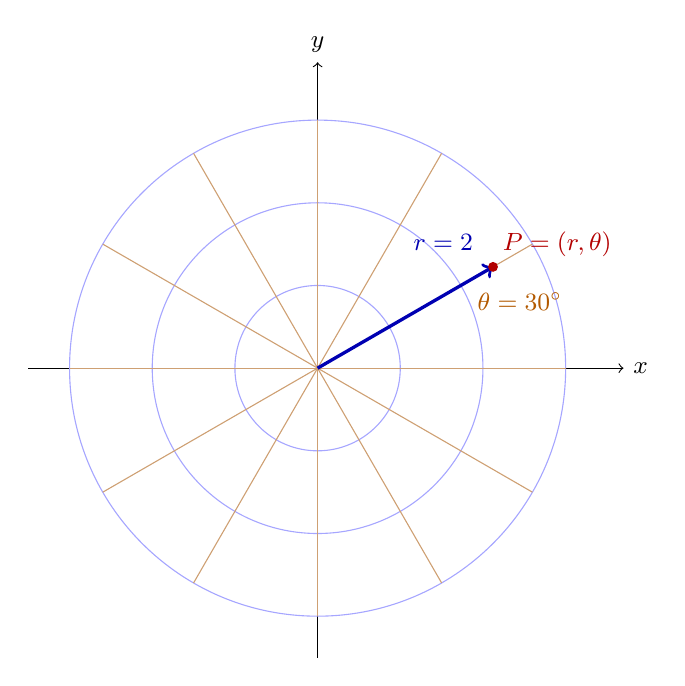
\begin{tikzpicture}[scale=1.05, every node/.style={font=\small}]
    \draw[->] (-3.5,0) -- (3.7,0) node[right] {$x$};
    \draw[->] (0,-3.5) -- (0,3.7) node[above] {$y$};
    \foreach \radio in {1,2,3}{
        \draw[blue!35] (0,0) circle (\radio);
    }
    \foreach \angulo in {0,30,...,330}{
        \draw[orange!65!black!55] (0,0) -- (\angulo:3);
    }
    \draw[->, very thick, blue!70!black] (0,0) -- (30:2.45);
    \fill[red!70!black] (30:2.45) circle (1.7pt) node[above right] {$P=(r,\theta)$};
    \node[blue!70!black] at (45:2.15) {$r=2$};
    \node[orange!70!black, yshift=-10pt] at (25:2.7) {$\theta=30^\circ$};
\end{tikzpicture}
\end{center}

Por ejemplo, todos los puntos de la circunferencia $r=2$ están a distancia $2$ del origen. Todos los puntos sobre el rayo $\theta=30^\circ$ tienen la misma dirección, aunque estén a distintas distancias.

\subsection{Componentes de un punto en polares}

El segmento de longitud $r$ que va del origen a $P$ forma un triángulo rectángulo con sus proyecciones sobre los ejes. Por trigonometría,
\[
\cos\theta=\frac{x}{r},
\qquad
\sin\theta=\frac{y}{r}.
\]
De aquí salen las dos componentes rectangulares del vector de posición:
\[
x=r\cos\theta,
\qquad
y=r\sin\theta.
\]
Es decir, $r\cos\theta$ es la parte horizontal y $r\sin\theta$ es la parte vertical.

También es útil nombrar dos direcciones unitarias:
\[
\mathbf{e}_r=\langle\cos\theta,\sin\theta\rangle,
\qquad
\mathbf{e}_\theta=\langle-\sin\theta,\cos\theta\rangle.
\]
El vector $\mathbf{e}_r$ apunta directamente hacia afuera del origen; $\mathbf{e}_\theta$ es perpendicular a él y apunta en el sentido en que aumenta el ángulo. A diferencia de los vectores unitarios rectangulares, estas direcciones cambian al movernos de un punto a otro.

\subsection{Conversión entre coordenadas rectangulares y polares}

\subsubsection*{De polares a rectangulares}

Si conocemos $(r,\theta)$, usamos las proyecciones anteriores:
\[
\boxed{x=r\cos\theta, y=r\sin\theta.}
\]
\textbf{Ejemplo.} Si $P=(3,7\pi/6)$, entonces
\[
x=3\cos\left(\frac{7\pi}{6}\right)=-\frac{3\sqrt{3}}{2},
\qquad
y=3\sin\left(\frac{7\pi}{6}\right)=-\frac{3}{2}.
\]
Por tanto, en coordenadas rectangulares $P=\left(-\dfrac{3\sqrt{3}}{2},-\dfrac{3}{2}\right)$.

\subsubsection*{De rectangulares a polares}

Si conocemos $(x,y)$, la distancia al origen se obtiene con el teorema de Pitágoras:
\[
\boxed{r=\sqrt{x^2+y^2}.}
\]
Para el ángulo se puede usar
\[
\tan\theta=\frac{y}{x}.
\]
Al usar esta última fórmula hay que revisar el cuadrante en el que está el punto, porque la tangente tiene el mismo valor en direcciones opuestas.

\textbf{Ejemplo.} Sea $Q=(-\sqrt{3},1)$. Entonces
\[
r=\sqrt{(-\sqrt{3})^2+1^2}=2.
\]
Además, $\tan\theta=-\dfrac{1}{\sqrt{3}}$. Como $Q$ está en el segundo cuadrante, el ángulo correcto es $\theta=5\pi/6$. Así,
\[
Q=(-\sqrt{3},1)=\left(2,\frac{5\pi}{6}\right).
\]

En el origen se tiene $r=0$, pero el ángulo no está definido: cualquier dirección lleva al mismo punto. Por esta razón, el origen debe tratarse con cuidado cuando se usan fórmulas que contienen $\theta$.

\section{Coordenadas cilíndricas}

Las coordenadas cilíndricas extienden las coordenadas polares al espacio. Para localizar un punto, primero se usa su posición polar sobre el plano $xy$ y luego se indica su altura. Son especialmente útiles cuando un objeto tiene simetría alrededor del eje $z$, como una tubería, un tanque o un cilindro.

\begin{mydefinition}{Coordenadas cilíndricas}
Las coordenadas cilíndricas de un punto $P$ se escriben $(r,\theta,z)$, donde:
\begin{itemize}
    \item $r$ es la distancia de $P$ al eje $z$; equivale a la distancia de la proyección de $P$ al origen en el plano $xy$.
    \item $\theta$ es el ángulo de esa proyección, medido desde el eje positivo $x$.
    \item $z$ es la altura del punto, igual que en las coordenadas rectangulares.
\end{itemize}
\end{mydefinition}

\subsection{Cómo intuirlas geométricamente}

Una forma sencilla de pensar en $(r,\theta,z)$ es la siguiente: baja el punto hasta el plano $xy$, localiza allí su posición polar $(r,\theta)$ y después súbelo una altura $z$. El conjunto de puntos que tienen el mismo valor de $r$ forma un cilindro alrededor del eje $z$.

\begin{center}
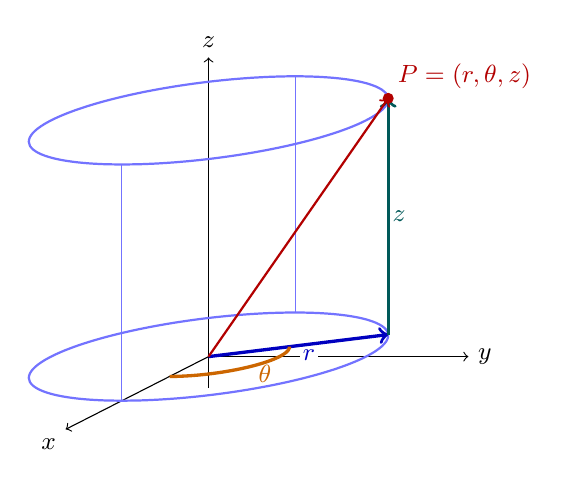
\begin{tikzpicture}[x={(-0.55cm,-0.28cm)}, y={(1cm,0cm)}, z={(0cm,1cm)}, scale=1, every node/.style={font=\small}]
    \draw[->] (0,0,0) -- (3.3,0,0) node[below left] {$x$};
    \draw[->] (0,0,0) -- (0,3.3,0) node[right] {$y$};
    \draw[->] (0,0,-0.4) -- (0,0,3.8) node[above] {$z$};
    \draw[blue!55, thick] plot[smooth cycle, domain=0:360, samples=60]
        ({2*cos(\x)}, {2*sin(\x)}, 0);
    \draw[blue!55, thick] plot[smooth cycle, domain=0:360, samples=60]
        ({2*cos(\x)}, {2*sin(\x)}, 3);
    \draw[blue!55] (2,0,0) -- (2,0,3);
    \draw[blue!55] (-2,0,0) -- (-2,0,3);
    % El punto P tiene r=2, por lo que está sobre la superficie del cilindro.
    \coordinate (B) at (-1,1.732,0);
    \coordinate (P) at (-1,1.732,3);
    \draw[->, very thick, blue!75!black] (0,0,0) -- (B)
        node[midway, below right, fill=white, inner sep=1pt] {$r$};
    \draw[->, very thick, teal!70!black] (B) -- (P)
        node[midway, right, fill=white, inner sep=1pt] {$z$};
    \draw[->, thick, red!70!black] (0,0,0) -- (P);
    \draw[orange!80!black, very thick] plot[domain=0:120, samples=40]
        ({0.9*cos(\x)}, {0.9*sin(\x)}, 0);
    \node[orange!80!black, inner sep=1pt, yshift=-2pt] at ({1.15*cos(62)}, {1.15*sin(62)}, 0) {$\theta$};
    \fill[red!70!black] (P) circle (2pt) node[above right] {$P=(r,\theta,z)$};
\end{tikzpicture}
\end{center}

En la figura, el punto $B$ es la proyección de $P$ sobre el plano $xy$. El segmento azul $OB$ mide $r$ y llega hasta la superficie del cilindro; el segmento verde $BP$ mide la altura $z$. El arco naranja muestra el ángulo $\theta$ y el vector rojo une el origen con el punto $P$.

\subsection{Componentes y superficies coordenadas}

Las componentes rectangulares del punto se obtienen aplicando las fórmulas polares en el plano $xy$ y conservando la altura:
\[
x=r\cos\theta,
\qquad
y=r\sin\theta,
\qquad
z=z.
\]
Las tres coordenadas describen familias de superficies sencillas:
\begin{itemize}
    \item $r=\text{constante}$ representa un cilindro circular alrededor del eje $z$.
    \item $\theta=\text{constante}$ representa un semiplano vertical que contiene al eje $z$.
    \item $z=\text{constante}$ representa un plano horizontal.
\end{itemize}

\subsection{Conversión cilíndrica--rectangular}

\subsubsection*{De cilíndricas a rectangulares}

\[
\boxed{x=r\cos\theta,\qquad y=r\sin\theta,\qquad z=z.}
\]
\textbf{Ejemplo.} Para $P=(2,\pi/3,-1)$,
\[
x=2\cos\left(\frac{\pi}{3}\right)=1,
\qquad
y=2\sin\left(\frac{\pi}{3}\right)=\sqrt{3}.
\]
Por tanto, $P=(1,\sqrt{3},-1)$ en coordenadas rectangulares.

\subsubsection*{De rectangulares a cilíndricas}

\[
\boxed{r=\sqrt{x^2+y^2},\qquad \theta=\operatorname{atan2}(y,x),\qquad z=z.}
\]
El ángulo se obtiene igual que en coordenadas polares; hay que tomar en cuenta el cuadrante de la proyección sobre el plano $xy$.

\textbf{Ejemplo.} Para $Q=(-1,\sqrt{3},4)$,
\[
r=\sqrt{(-1)^2+(\sqrt{3})^2}=2,
\qquad
\theta=\frac{2\pi}{3}.
\]
Así, $Q=\left(2,\dfrac{2\pi}{3},4\right)$ en coordenadas cilíndricas.

\section{Coordenadas esféricas}

Las coordenadas esféricas describen un punto del espacio usando su distancia al origen y dos ángulos. Son naturales cuando el problema involucra esferas, ondas que se propagan desde una fuente o campos que apuntan hacia afuera o hacia adentro del origen.

\begin{mydefinition}{Coordenadas esféricas}
Usaremos la convención $(\rho,\theta,\varphi)$, donde:
\begin{itemize}
    \item $\rho$ es la distancia del origen al punto $P$.
    \item $\theta$ es el ángulo de la proyección de $P$ sobre el plano $xy$, medido desde el eje positivo $x$.
    \item $\varphi$ es el ángulo medido desde el eje positivo $z$ hasta el segmento que une el origen con $P$.
\end{itemize}
Normalmente se toma $\rho\geq 0$, $0\leq\theta<2\pi$ y $0\leq\varphi\leq\pi$.
\end{mydefinition}

\subsection{Cómo intuirlas geométricamente}

Imagina una esfera centrada en el origen. Primero se elige una dirección horizontal con $\theta$; después se inclina esa dirección mediante $\varphi$ y, por último, se avanza una distancia $\rho$. De este modo, $(\rho,\theta,\varphi)$ localiza cualquier punto fuera del origen.

\begin{center}
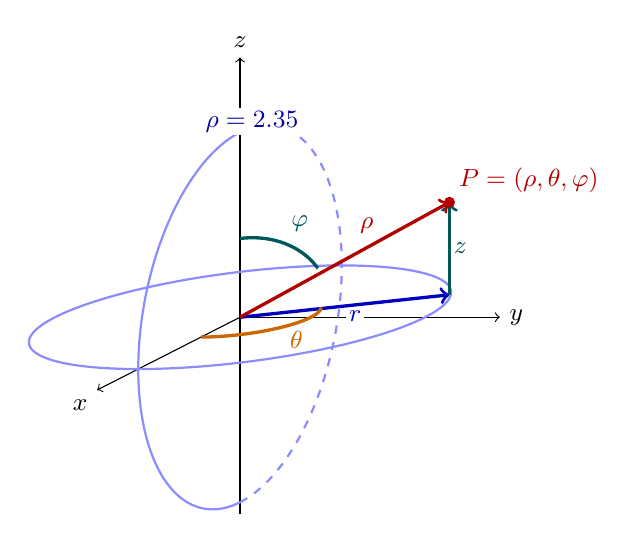
\begin{tikzpicture}[x={(-0.55cm,-0.28cm)}, y={(1cm,0cm)}, z={(0cm,1cm)}, scale=1, every node/.style={font=\small}]
    \draw[->] (0,0,0) -- (3.3,0,0) node[below left] {$x$};
    \draw[->] (0,0,0) -- (0,3.3,0) node[right] {$y$};
    \draw[->] (0,0,-2.5) -- (0,0,3.3) node[above] {$z$};
    \draw[blue!45, thick] plot[smooth cycle, domain=0:360, samples=70]
        ({2.35*cos(\x)}, {2.35*sin(\x)}, 0);
    \draw[blue!45, thick] plot[smooth, domain=0:180, samples=45]
        ({2.35*sin(\x)}, 0, {2.35*cos(\x)});
    \draw[blue!45, dashed, thick] plot[smooth, domain=180:360, samples=45]
        ({2.35*sin(\x)}, 0, {2.35*cos(\x)});
    \coordinate (B) at (-1.018,2.1,0);
    \coordinate (P) at (-1.018,2.1,1.175);
    \draw[->, very thick, blue!75!black] (0,0,0) -- (B)
        node[midway, below right, fill=white, inner sep=1pt] {$r$};
    \draw[->, very thick, teal!70!black] (B) -- (P)
        node[midway, right, fill=white, inner sep=1pt] {$z$};
    \draw[->, very thick, red!70!black] (0,0,0) -- (P)
        node[midway, above right, inner sep=1pt, yshift=8pt, xshift=4pt] {$\rho$};
    \draw[orange!80!black, very thick] plot[domain=0:120, samples=40]
        ({0.9*cos(\x)}, {0.9*sin(\x)}, 0);
    \node[orange!80!black, inner sep=1pt, yshift=-4pt] at ({1.15*cos(62)}, {1.15*sin(62)}, 0) {$\theta$};
    \draw[teal!70!black, very thick] plot[domain=0:60, samples=35]
        ({1.0*sin(\x)*cos(120)}, {1.0*sin(\x)*sin(120)}, {1.0*cos(\x)});
    \node[teal!70!black, inner sep=1pt, above left, yshift=10pt, xshift=-5pt] at (-0.48,0.82,0.56) {$\varphi$};
    \fill[red!70!black] (P) circle (2pt) node[above right] {$P=(\rho,\theta,\varphi)$};
    \node[blue!65!black, fill=white, inner sep=1pt] at (-1.55,-0.7,2.05) {$\rho=2.35$};
\end{tikzpicture}
\end{center}

El punto $B$ es la proyección de $P$ sobre el plano $xy$. El segmento azul $OB$ mide $r=\rho\sin\varphi$, el segmento verde $BP$ mide $z=\rho\cos\varphi$ y el vector rojo $OP$ mide $\rho$. El arco naranja corresponde a $\theta$ y el arco verde azulado corresponde a $\varphi$.

\subsection{Componentes y superficies coordenadas}

El triángulo formado por $\rho$, su proyección $r$ sobre el plano $xy$ y la altura $z$ da
\[
r=\rho\sin\varphi,
\qquad
z=\rho\cos\varphi.
\]
Después, al descomponer $r$ sobre los ejes $x$ y $y$, se obtiene
\[
x=\rho\sin\varphi\cos\theta,
\qquad
y=\rho\sin\varphi\sin\theta,
\qquad
z=\rho\cos\varphi.
\]
Las superficies de coordenada constante son:
\begin{itemize}
    \item $\rho=\text{constante}$: una esfera centrada en el origen.
    \item $\theta=\text{constante}$: un semiplano vertical que contiene al eje $z$.
    \item $\varphi=\text{constante}$: un cono con vértice en el origen.
\end{itemize}

\subsection{Conversión esférica--rectangular}

\subsubsection*{De esféricas a rectangulares}

\[
\boxed{
x=\rho\sin\varphi\cos\theta,
\qquad
y=\rho\sin\varphi\sin\theta,
\qquad
z=\rho\cos\varphi.}
\]
\textbf{Ejemplo.} Sea $P=(4,\pi/6,\pi/3)$. Entonces
\begin{align*}
x&=4\left(\frac{\sqrt{3}}{2}\right)\left(\frac{\sqrt{3}}{2}\right)=3,\\
y&=4\left(\frac{\sqrt{3}}{2}\right)\left(\frac{1}{2}\right)=\sqrt{3},\\
z&=4\left(\frac{1}{2}\right)=2.
\end{align*}
Así, $P=(3,\sqrt{3},2)$ en coordenadas rectangulares.

\subsubsection*{De rectangulares a esféricas}

Primero se calcula la distancia al origen y la distancia al eje $z$:
\[
\rho=\sqrt{x^2+y^2+z^2},
\qquad
r=\sqrt{x^2+y^2}.
\]
Luego,
\[
\boxed{
\theta=\operatorname{atan2}(y,x),
\qquad
\varphi=\arccos\left(\frac{z}{\rho}\right).}
\]
\textbf{Ejemplo.} Para $Q=(-\sqrt{3},3,2)$,
\[
\rho=\sqrt{3+9+4}=4,
\qquad
\theta=\frac{2\pi}{3},
\qquad
\varphi=\arccos\left(\frac{2}{4}\right)=\frac{\pi}{3}.
\]
Por tanto,
\[
Q=(-\sqrt{3},3,2)=\left(4,\frac{2\pi}{3},\frac{\pi}{3}\right).
\]

En el origen $\rho=0$ y los ángulos no están definidos. Cerca del origen conviene revisar con cuidado las expresiones que contienen $\theta$ o $\varphi$.

\subsection{Ejercicios}

Los ejercicios avanzan desde conversiones directas hasta la descripción de superficies y sólidos.
\begin{enumerate}
    \item Convierta los siguientes puntos de coordenadas polares a rectangulares:
\[
(2,0),\qquad \left(2,\frac{\pi}{2}\right),\qquad (2,\pi),\qquad \left(2,\frac{3\pi}{2}\right).
\]
Ubique los cuatro puntos en un plano cartesiano.

    \item Convierta cada punto de coordenadas rectangulares a polares, con $r\geq 0$ y $0\leq\theta<2\pi$:
\begin{enumerate}
    \item $(1,\sqrt{3})$.
    \item $(-\sqrt{3},1)$.
    \item $(-1,-1)$.
\end{enumerate}

    \item Sea $P=(3,\pi/6)$ en coordenadas polares.
\begin{enumerate}
    \item Convierta $P$ a coordenadas rectangulares.
    \item Escriba otras dos parejas de coordenadas polares que representen el mismo punto.
    \item Explique por qué $(3,13\pi/6)$ representa el mismo punto que $P$.
\end{enumerate}

    \item Convierta los siguientes puntos de coordenadas cilíndricas $(r,\theta,z)$ a rectangulares:
\begin{enumerate}
    \item $(3,0,2)$.
    \item $\left(2,\frac{\pi}{2},-1\right)$.
    \item $\left(4,\frac{5\pi}{6},0\right)$.
\end{enumerate}

    \item Convierta los siguientes puntos de coordenadas rectangulares a cilíndricas. Use $r\geq 0$ y $0\leq\theta<2\pi$.
\begin{enumerate}
    \item $(1,\sqrt{3},3)$.
    \item $(-2,0,-1)$.
    \item $(0,-3,4)$.
\end{enumerate}

    \item Describa geométricamente cada una de las siguientes superficies en coordenadas cilíndricas. Incluya un dibujo sencillo en cada caso.
\begin{enumerate}
    \item $r=2$.
    \item $\theta=\pi/4$.
    \item $z=-3$.
\end{enumerate}

    \item Considere el sólido descrito en coordenadas cilíndricas por
\[
0\leq r\leq 2,\qquad 0\leq\theta<2\pi,\qquad 0\leq z\leq 3.
\]
\begin{enumerate}
    \item Describa el sólido con palabras y haga un dibujo.
    \item Escriba una desigualdad equivalente en coordenadas rectangulares.
    \item Determine si el punto $(1,1,2)$ pertenece al sólido.
\end{enumerate}

    \item Convierta los siguientes puntos de coordenadas esféricas $(\rho,\theta,\varphi)$ a rectangulares. Recuerde que $\varphi$ se mide desde el eje positivo $z$.
\begin{enumerate}
    \item $\left(2,0,\frac{\pi}{2}\right)$.
    \item $\left(4,\frac{\pi}{2},\frac{\pi}{3}\right)$.
    \item $(3,\pi,\pi/2)$.
\end{enumerate}

    \item Convierta el punto $P=(3,3,3\sqrt{2})$ de coordenadas rectangulares a esféricas.
\begin{enumerate}
    \item Calcule $\rho$.
    \item Determine $\theta$ a partir de la proyección sobre el plano $xy$.
    \item Determine $\varphi$ usando la componente $z$.
    \item Verifique el resultado convirtiéndolo de nuevo a coordenadas rectangulares.
\end{enumerate}

    \item Sea $P=(-3,3,3\sqrt{2})$.
\begin{enumerate}
    \item Exprese $P$ en coordenadas cilíndricas.
    \item Exprese $P$ en coordenadas esféricas, usando la convención de estos apuntes.
    \item Compruebe que las dos respuestas tienen el mismo ángulo $\theta$.
    \item Explique cuál de los dos sistemas describe más directamente la distancia de $P$ al origen y cuál describe más directamente su altura sobre el plano $xy$.
\end{enumerate}

\end{enumerate}
